% !TeX root = ../main.tex

\section*{Parzen-Window estimator}
\paragraph{Idea:} Quantify the number of samples with a appropriate kernel/window function. In other words we interpolate
% \footnote{General remark: We obtain a continuous pdf, i.e.\ desity estimation converts a list of measurments to a statistical model}
the pdf from the observations in the neighbourhood of a position $\vec{x}$.

\paragraph{Derivation:} We can express $p_R$, the probability that $\vec{x}$ lies within a region $R$, in terms of the volume $V_R$ of this region\footnote{$\int_R \,d\vec{x}$ is just the volume of $R$, we also write $V_R$ for the volume}, when $p(\vec{x})$ is approximately constant in $R$.

\begin{equation*}
  p_R = \int_R p(\vec{x}) \,d\vec{x} \ \approx \ p(\vec{x}) \int_R \,d\vec{x} = p(\vec{x}) V_R
\end{equation*}

We determine $p_R = \dfrac{k_R}{N}$ the probability of making observations in region $R$ (also ``relative frequency'')  by counting the samples in $R$ ($=k_R$) and dividing by the total number of samples.

\begin{equation*}
  p(\vec{x}) = \dfrac{p_R}{V_R} = \dfrac{k_R}{V_R N}
\end{equation*}

Let's write the parzen window estimator as a function of a kernel $k(\vec{x}; \vec{x_i})$. If $R$ is a d-dimensional hypercube with side length $h$, then its volume is $h^d$.

\begin{equation*}
  \boxed{p(\vec{x}) = \dfrac{1}{h^d N} \sum_{i=1}^N k(\vec{x}; \vec{x_i})}
\end{equation*}

where we can choose a suitable kernel function $k(\vec{x}; \vec{x_i})$. E.g. binary decision\footnote{$\vec{x_i}$ and $\vec{x}$ are not father apart then $0.5 h$ in any dimension $k$} or a (multivariate) gaussian kernel\footnote{Omit $h^d$ if the kernel is gaussian}:

\begin{equation*}
  k(\vec{x}; \vec{x_i}) = \begin{cases}
    1 &\text{when } \dfrac{|x_{i,k} - x_k|}{h} \le \dfrac{1}{2}\\
    0 &\text{otherwise}
  \end{cases}
  \qquad \qquad
  k(\vec{x}; \vec{x_i}) = \dfrac{1}{{(2\pi)}^d |\Sigma|} e^{-{(\vec{x} - \vec{x_i})}^T \Sigma^{-1}(\vec{x}-\vec{x_i})}
\end{equation*}

\begin{figure}[H]
  \centering
  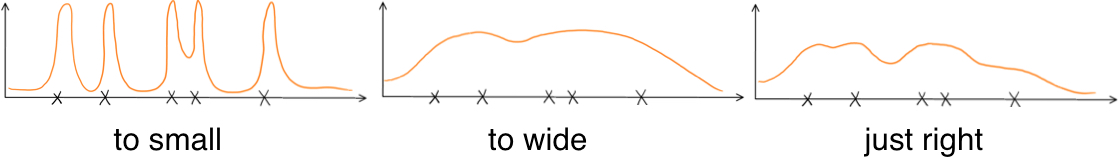
\includegraphics[width=\textwidth]{03-window-size}
  \caption{Effects of the window / kernel size}
  % TODO: change to to too small
\end{figure}

\paragraph{How can we determine a good window / kernel size} $\hat{h}$?

Let's do ML est.\ with a cross-validation (cv) e.g.\ leave-one-sample-out cv. Estimate the pdf from all samples except $\vec{x_j}$, which will be used to evaluate the quality of the pdf using window size $h$.

\begin{equation*}
  p_{h,N-1}^j(\vec{x}) = \dfrac{1}{h^d N} \sum_{i=1 (i \neq j)}^N k(\vec{x}; \vec{x_i})
\end{equation*}

\begin{equation*}
  \hat{h} = \argmax_h L(h) = \argmax_h \prod_{j=1}^N p_{h,N-1}^j(\vec{x_j}) = \argmax_h \sum_{j=1}^N \log p_{h,N-1}^j(\vec{x_j})
\end{equation*}

The position of the maximum does not change (when using log-likelihood), because the logarithm is a strictly monotonic function.

\paragraph{Remark:}
When the data is scaled differently, then we would like the window size to be adaptive. One solution is to use the k-NN combined with the parzen window estimator. This means we foce the number of neighours inside a window to equal a fixed k.
